% Options for packages loaded elsewhere
\PassOptionsToPackage{unicode}{hyperref}
\PassOptionsToPackage{hyphens}{url}
%
\documentclass[
  english,
  man,floatsintext]{apa6}
\usepackage{lmodern}
\usepackage{amssymb,amsmath}
\usepackage{ifxetex,ifluatex}
\ifnum 0\ifxetex 1\fi\ifluatex 1\fi=0 % if pdftex
  \usepackage[T1]{fontenc}
  \usepackage[utf8]{inputenc}
  \usepackage{textcomp} % provide euro and other symbols
\else % if luatex or xetex
  \usepackage{unicode-math}
  \defaultfontfeatures{Scale=MatchLowercase}
  \defaultfontfeatures[\rmfamily]{Ligatures=TeX,Scale=1}
\fi
% Use upquote if available, for straight quotes in verbatim environments
\IfFileExists{upquote.sty}{\usepackage{upquote}}{}
\IfFileExists{microtype.sty}{% use microtype if available
  \usepackage[]{microtype}
  \UseMicrotypeSet[protrusion]{basicmath} % disable protrusion for tt fonts
}{}
\makeatletter
\@ifundefined{KOMAClassName}{% if non-KOMA class
  \IfFileExists{parskip.sty}{%
    \usepackage{parskip}
  }{% else
    \setlength{\parindent}{0pt}
    \setlength{\parskip}{6pt plus 2pt minus 1pt}}
}{% if KOMA class
  \KOMAoptions{parskip=half}}
\makeatother
\usepackage{xcolor}
\IfFileExists{xurl.sty}{\usepackage{xurl}}{} % add URL line breaks if available
\IfFileExists{bookmark.sty}{\usepackage{bookmark}}{\usepackage{hyperref}}
\hypersetup{
  pdftitle={The Sound of Teaching Music: Expert Pianists' Performance Modulations for Novices},
  pdflang={en-EN},
  pdfkeywords={teaching, expertise, skill transmission, artistic expression, music},
  hidelinks,
  pdfcreator={LaTeX via pandoc}}
\urlstyle{same} % disable monospaced font for URLs
\usepackage{graphicx}
\makeatletter
\def\maxwidth{\ifdim\Gin@nat@width>\linewidth\linewidth\else\Gin@nat@width\fi}
\def\maxheight{\ifdim\Gin@nat@height>\textheight\textheight\else\Gin@nat@height\fi}
\makeatother
% Scale images if necessary, so that they will not overflow the page
% margins by default, and it is still possible to overwrite the defaults
% using explicit options in \includegraphics[width, height, ...]{}
\setkeys{Gin}{width=\maxwidth,height=\maxheight,keepaspectratio}
% Set default figure placement to htbp
\makeatletter
\def\fps@figure{htbp}
\makeatother
\setlength{\emergencystretch}{3em} % prevent overfull lines
\providecommand{\tightlist}{%
  \setlength{\itemsep}{0pt}\setlength{\parskip}{0pt}}
\setcounter{secnumdepth}{-\maxdimen} % remove section numbering
% Make \paragraph and \subparagraph free-standing
\ifx\paragraph\undefined\else
  \let\oldparagraph\paragraph
  \renewcommand{\paragraph}[1]{\oldparagraph{#1}\mbox{}}
\fi
\ifx\subparagraph\undefined\else
  \let\oldsubparagraph\subparagraph
  \renewcommand{\subparagraph}[1]{\oldsubparagraph{#1}\mbox{}}
\fi
% Manuscript styling
\usepackage{upgreek}
\captionsetup{font=singlespacing,justification=justified}

% Table formatting
\usepackage{longtable}
\usepackage{lscape}
% \usepackage[counterclockwise]{rotating}   % Landscape page setup for large tables
\usepackage{multirow}		% Table styling
\usepackage{tabularx}		% Control Column width
\usepackage[flushleft]{threeparttable}	% Allows for three part tables with a specified notes section
\usepackage{threeparttablex}            % Lets threeparttable work with longtable

% Create new environments so endfloat can handle them
% \newenvironment{ltable}
%   {\begin{landscape}\begin{center}\begin{threeparttable}}
%   {\end{threeparttable}\end{center}\end{landscape}}
\newenvironment{lltable}{\begin{landscape}\begin{center}\begin{ThreePartTable}}{\end{ThreePartTable}\end{center}\end{landscape}}

% Enables adjusting longtable caption width to table width
% Solution found at http://golatex.de/longtable-mit-caption-so-breit-wie-die-tabelle-t15767.html
\makeatletter
\newcommand\LastLTentrywidth{1em}
\newlength\longtablewidth
\setlength{\longtablewidth}{1in}
\newcommand{\getlongtablewidth}{\begingroup \ifcsname LT@\roman{LT@tables}\endcsname \global\longtablewidth=0pt \renewcommand{\LT@entry}[2]{\global\advance\longtablewidth by ##2\relax\gdef\LastLTentrywidth{##2}}\@nameuse{LT@\roman{LT@tables}} \fi \endgroup}

% \setlength{\parindent}{0.5in}
% \setlength{\parskip}{0pt plus 0pt minus 0pt}

% \usepackage{etoolbox}
\makeatletter
\patchcmd{\HyOrg@maketitle}
  {\section{\normalfont\normalsize\abstractname}}
  {\section*{\normalfont\normalsize\abstractname}}
  {}{\typeout{Failed to patch abstract.}}
\makeatother
\shorttitle{The Sound of Teaching Music}
\author{Atsuko Tominaga\textsuperscript{1}, Günther Knoblich\textsuperscript{1}, \& Natalie Sebanz\textsuperscript{1}}
\affiliation{
\vspace{0.5cm}
\textsuperscript{1} Department of Cognitive Science, Central European University}
\authornote{

Correspondence concerning this article should be addressed to Atsuko Tominaga, Quellenstraße 51, 1100 Vienna, Austria. E-mail: Tominaga\_Atsuko@phd.ceu.edu}
\keywords{teaching, expertise, skill transmission, artistic expression, music\newline\indent Word count: X}
\usepackage{csquotes}
\ifxetex
  % Load polyglossia as late as possible: uses bidi with RTL langages (e.g. Hebrew, Arabic)
  \usepackage{polyglossia}
  \setmainlanguage[]{english}
\else
  \usepackage[shorthands=off,main=english]{babel}
\fi
\ifluatex
  \usepackage{selnolig}  % disable illegal ligatures
\fi
\newlength{\cslhangindent}
\setlength{\cslhangindent}{1.5em}
\newenvironment{cslreferences}%
  {\setlength{\parindent}{0pt}%
  \everypar{\setlength{\hangindent}{\cslhangindent}}\ignorespaces}%
  {\par}

\title{The Sound of Teaching Music: Expert Pianists' Performance Modulations for Novices}

\date{}

\abstract{
aaaa
}

\begin{document}
\maketitle

\hypertarget{introduction}{%
\section{1. Introduction}\label{introduction}}

Deliberate teaching has supported human skill transmission over generations and provides a key route for learning (Tomasello, 2016; Whiten, 2017). Experts modulate their behaviour so that novices can extract relevant information to learn a novel skill. In particular, adults modulate their speech (motherese) and actions (motionese) when demonstrating a skill to infant learners (Brand, Baldwin, \& Ashburn, 2002; Fernald, 1985). These modulations include slowing down and exaggerating sounds and actions. Similar findings were obtained in studies with adult learners, where exaggerations were observed when native British English speakers were talking to first language English learners (Uther, Knoll, \& Burnham, 2007) and when skilled adults were teaching xylophone melodies to novices (McEllin, Knoblich, \& Sebanz, 2017). The observed modulations are thought to provide communicative signals that can facilitate learning by affecting attention and memory (Csibra \& Gergely, 2009).

Previous research has shown that demonstrators not only adjust their gestures (Campisi \& Özyürek, 2013) and actions (Fukuyama et al., 2015) to learners' skills but engage in specific action modulations to highlight particular aspects of demonstrated actions. For example, Schaik, Meyer, Ham, and Hunnius (2019) showed that adults used specific action modulations for demonstrating different action effects of objects to infants. Ho, Littman, MacGlashan, Cushman, and Austerweil (2016) found that demonstrators chose costly movement paths at structurally important points to disambiguate one goal over other possibilities.

Importantly, in some domains teaching requires not only demonstrating \emph{what} to do, but \emph{how} to perform actions. In artistic contexts, novices need to learn how exactly to perform actions by relying on particular techniques (Sloboda, 2000). For example, when playing a piece of music on the piano, it is not sufficient to press the keys in the correct order, but learners need to be able to implement expressive techniques (Juslin, 2003). This raises the question of whether and how experts modulate their actions during demonstration in artistic contexts, where expressivity is an integral part of what learners need to acquire. Studying action modulations that serve the teaching of artistic techniques is of broader theoretical importance: It can show whether action modulations can be used to selectively highlight subtle aspects of actions that define expert performance.

In the present study, we employed musical expressive techniques as skills to be taught because multiple properties of the performance (e.g., timing, articulation, loudness) can be modulated at the same time. Specific and subtle aspects of the performance need to be highlighted to teach a respective technique. We asked whether skilled pianists use sound to communicate didactic intentions. Pianists were asked to perform a piece in order to demonstrate to a learner how to implement the notated expressions (teaching condition) and to play the same piece for an audience (performing condition). Two basic expressive techniques in piano performance were used: articulation (legato and staccato) and dynamics (forte and piano).

If experts rely on generic action modulations, it can be expected that they will play more slowly during demonstration, regardless of the kind of expressive techniques to be taught. To the extent that experts use action modulations to support their teaching of specific expressive techniques, they should produce longer legato and shorter staccato when teaching articulation whereas they should produce louder forte and softer piano when teaching dynamics. Furthermore, one could speculate that they might produce modulations specifically at structurally important points that best highlight the technique to be taught. Importantly, they should avoid modulating irrelevant properties of expression, e.g., the smoothness of the sound while teaching dynamics.

\clearpage

\hypertarget{experiment-1}{%
\section{2. Experiment 1}\label{experiment-1}}

\hypertarget{method}{%
\subsection{2.1. Method}\label{method}}

\hypertarget{participants}{%
\subsubsection{2.1.1. Participants}\label{participants}}

We recruited 36 piano experts who played the piano for at least the past 10 years or were studying piano performance at a music school at the time of recruitment. For data analysis, we excluded 5 participants due to experimental errors (3), an overall deviated tempo (2; outside 2 standard deviations from the average tempo across participants). Thirty-one participants (15 female) were included in data analysis. Most participants were right-handed (left; 2, both; 2). They had 12.45 years of practice on average (\emph{SD} = 5.66). All participants gave their informed consent before the experiment started and received vouchers for their participation. The study was approved by the United Ethical Review Committee for Research in Psychology (EPKEB) in Hungary.

\hypertarget{apparatus-and-stimuli}{%
\subsubsection{2.1.2. Apparatus and stimuli}\label{apparatus-and-stimuli}}

A weighted Yamaha MIDI digital piano was used to record participants' performance via Max/MSP on a MacBook Pro with MacOS X Mojave 10.14.3. The laptop and piano were connected to a high-fidelity soundcard (Focusrite Scarlett 6i6) to deliver a metronome and piano sound. All auditory feedback was given to participants through headphones (Audio-Technica ATH-M50X). Sheet music was displayed on a computer monitor in front of the participants. The pitch, onset and offset time of each note, and key velocity profiles were obtained from MIDI data using Max/MSP patchers.

One musical excerpt was used as a stimulus. The excerpt was taken from ``A Dozen a Day - Play with Ease in Many Keys" by Edna-Mae Burnam and modified for the experiment. It consisted of a 6-measure isochronous melody noted in 4/4 meter. The stimulus was composed in C major to be played with the right hand only. Non-expressive sheet music (i.e., sheet music without expressive notations; see \emph{Figure \ref{fig:stimuli}, A}) was used for the purpose of practice. Expressive notations were added to the non-expressive sheet music for the experiment. They referred to either articulation or dynamics (\emph{Figure \ref{fig:stimuli}, B-C}). Articulation was notated as either legato or staccato. Legato indicates that musical notes are to be connected and should sound smooth. Staccato requires producing musical notes with shortened duration, keeping them separate from each other. Dynamics was notated as either forte and piano. Forte indicates that musical notes should be played loudly whereas piano indicates that musical notes should be played softly. The notation did not include any indication of fingering (i.e., the positioning of the fingers when playing the piano) because the piece was simple and pilot testing had shown that specifying fingering was not required.

\hypertarget{procedure}{%
\subsubsection{2.1.3. Procedure}\label{procedure}}

In order to ensure that participants had sufficient motor skills to perform the piece, we asked them to practise the piece with the non-expressive sheet music (\emph{Figure \ref{fig:stimuli}, A}). Once they could perform the piece without pitch errors twice consecutively within 5 attempts, the experiment started.

First, participants were allocated to either the teaching or performing condition and asked to practise the excerpt with notated expressions of either articulation or dynamics (\emph{Figure \ref{fig:stimuli}, B-C}). As soon as they had produced the excerpt with notated expressions without pitch errors twice consecutively, the test trials began.

In the teaching condition, participants were instructed to play the excerpt of music as if they were teaching it to students. It was mentioned that the students already knew the sequence of the tones and that they were trying to learn how to perform the piece with a notated expression by listening to the participant's performance. In the performing condition, participants were asked to play the excerpt of music as if they were performing it to an audience (see details in \emph{\protect\hyperlink{supplemental}{Supplemental Materials}}). Participants played the piece 8 times per expressive technique per condition, so there were 32 trials in total (2 conditions x 2 expressive techniques x 8 trials). The order of the conditions was counterbalanced across participants. The order of the expressive techniques within each condition was also counterbalanced across participants. A leading metronome (80 beats per minute, 8 beats) indicated the target tempo before each trial.

At the end of the experiment, participants filled in a questionnaire asking about their demographic information and experience in piano performance/teaching.

\hypertarget{design-and-data-analysis}{%
\subsubsection{2.1.4. Design and data analysis}\label{design-and-data-analysis}}

The experiment had two factors; Condition (teaching vs.~performing) and Expressive Technique (articulation vs.~dynamics). Additionally, the factor Subcomponent was used when analysing data for each subcomponent for each technique separately (i.e., LS; legato vs.~staccato, FP; forte vs.~piano).

Three dependent variables were computed for data analysis. Interonset intervals (IOIs) are the intervals between onsets of adjacent notes and provide a tempo of tempo. Key-overlap time (KOT) is the difference between the offset time of the current tone (i.e., key release time) and the onset time of the ensuing tone, and measures the smoothness of musical sequences (Bresin \& Battel, 2000). A positive value indicates smooth legato styles due to overlap between the current and ensuing tone whereas a negative value indicates sharp staccato styles due to separation between the current and ensuing tone. Tone intensity is assessed by key velocity (KV) and measures the loudness of a musical note. The value of KV in MIDI varies between 0 (minimum) and 127 (maximum).

Data cleaning, preprocessing and statistical analysis were performed in R version 3.6.3. For statistical analysis, only 16th notes with expressive notations were included. Three trials were entirely excluded from data analysis because participants did not follow sheet music or complete performing till the end. Pitch errors were identified by comparing a sequence of musical notes produced by a participant with the sequence of musical notes according to the sheet music. Pitch errors included either extra, missing or substituted tones and were manually removed by using editData package. For onsets, 5.16\% of the trials contained at least one pitch error (extra notes; 2.78\%, missing notes; 2.24\%, substituted notes; 0.13\%). For offsets, 6.24\% of the trials contained at least one pitch error (extra notes; 2.78\%, missing notes; 2.29\%, substituted notes; 1.17\%). After we removed pitch errors, outliers for IOIs, KOT and KV were defined as values more than 3 standard deviations from the mean of each dependent variable and excluded from data analysis. Removed outliers were less than 5\% of overall responses for each dependent variable.

We performed separate analyses for the two expressive techniques (i.e., articulation, dynamics). A paired-sample \emph{t}-test or a Wilcoxon signed-rank tests (a non-parametric alternative to a paired \emph{t}-test) was performed to compare the mean IOIs in the teaching and performing condition. For KOT and KV, we performed a 2 x 2 repeated-measures analysis of variance (ANOVA) with the factors Condition (teaching vs.~performing) and Subcomponent (LS; legato vs.~staccato or FP; forte vs.~piano, respectively). The ``aov\_car" function in the afex package was used for a repeated-measures ANOVA. For post-hoc comparisons, we used emmeans package to investigate interactions from the ANOVA.

\begin{figure}
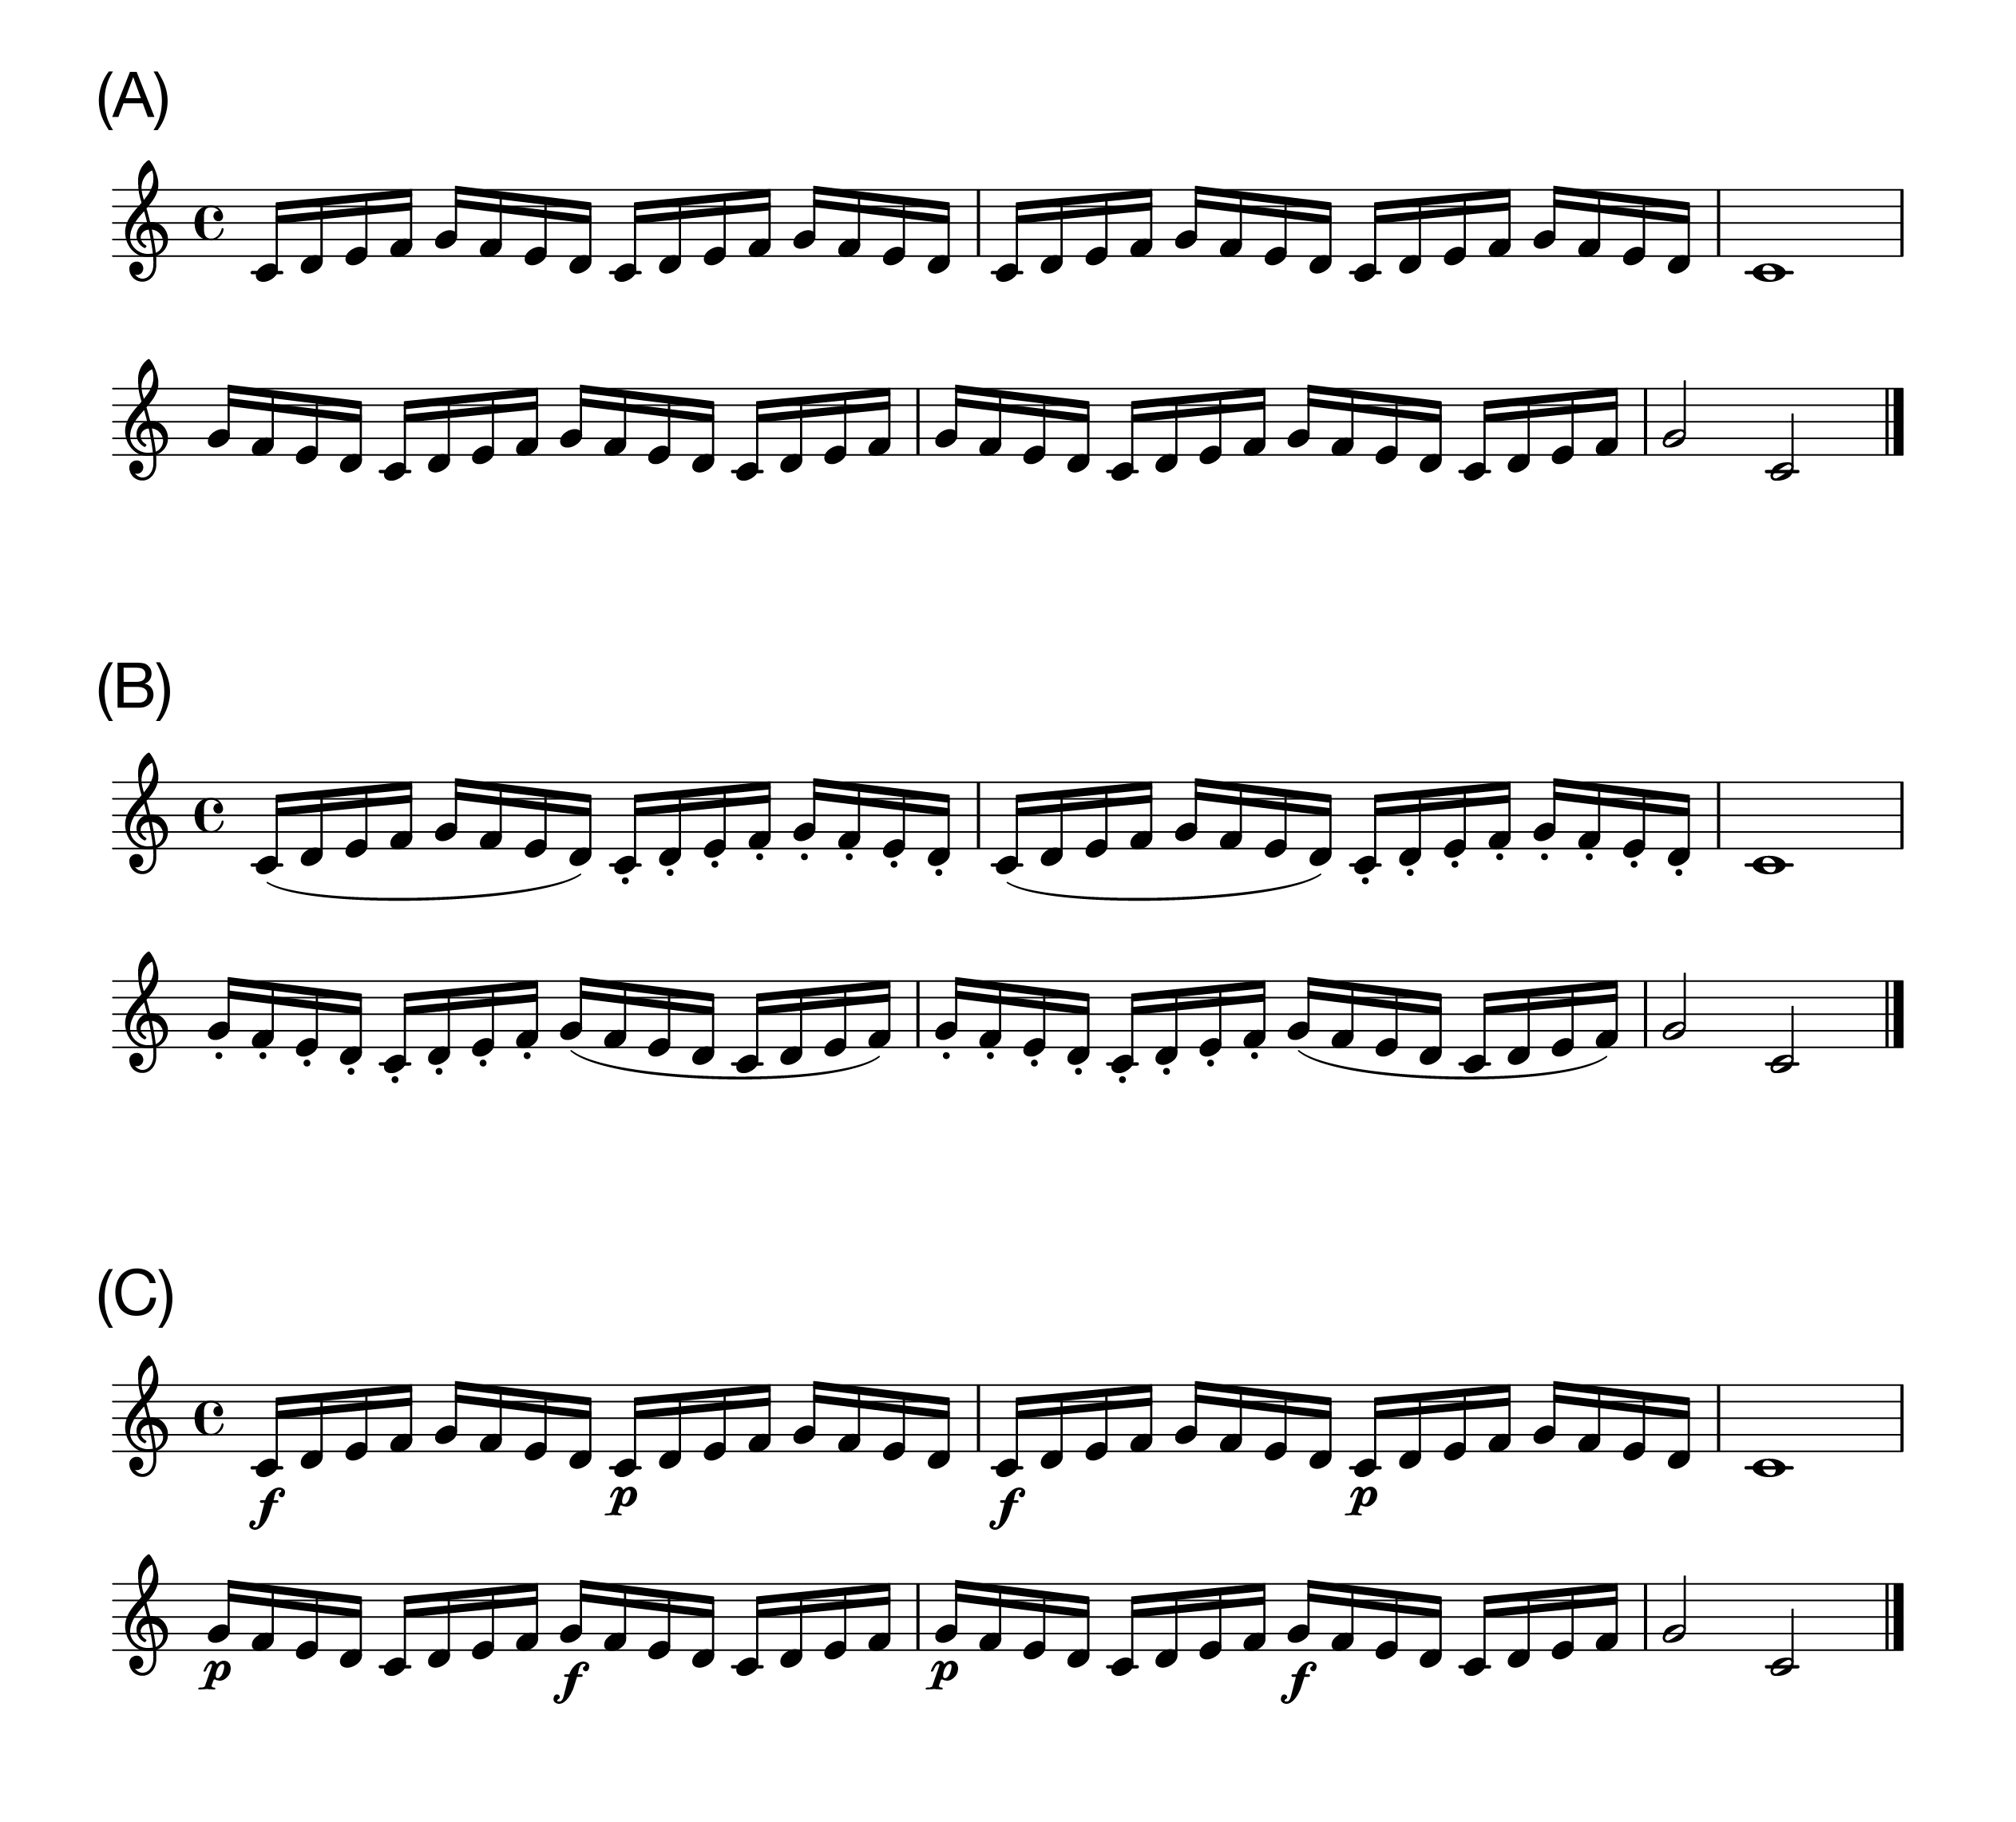
\includegraphics[width=1\linewidth]{manuscript_files/figure-latex/stim-1-1} \caption{\label{fig:stimuli}(A)Non-expressive sheet music. (B)Articulation. The curved line (slur) indicates legato and the dots indicate staccato. (C)Dynamics. The symbol `f' denotes forte and the symbol `p' denotes piano. For data analysis, only the 16th notes were included.}\label{fig:stim-1}
\end{figure}

\newpage

\hypertarget{results-articulation}{%
\subsection{2.2. Results (Articulation)}\label{results-articulation}}

All effects are reported as significant at \emph{p} \textless{} .05. We first report results for performance the piece with the notated expression of articulation (\emph{Figure \ref{fig:stimuli}, B}). followed by performance of the piece with the notated expression of dynamics (\emph{Figure \ref{fig:stimuli}, C}).

\hypertarget{interonset-intervals-iois}{%
\subsubsection{2.2.1. Interonset Intervals (IOIs)}\label{interonset-intervals-iois}}

In order to compare the mean IOIs between the teaching and performing condition, we conducted a Wiscoxon Signed-rank test, instead of a paired \emph{t}-test, because a Shapiro-Wilk test showed that the distribution of the mean difference was significantly different from the normal distribution. The Wiscoxon Signed-rank test revealed that participants played more slowly in the teaching condition {[}\emph{Mdn} = 189.55 (ms), \emph{IQR} = 26.74{]} than in the performing condition {[}\emph{Mdn} = 185.24 (ms), \emph{IQR} = 19.32{]} while playing the piece with notated articulation (\emph{p} = 0.021; \emph{Figure \ref{fig:ioi-1}}).

\hypertarget{key-overlap-time-kot}{%
\subsubsection{2.2.2. Key-Overlap Time (KOT)}\label{key-overlap-time-kot}}

Blah

\hypertarget{key-velocity-kv}{%
\subsubsection{2.2.3. Key Velocity (KV)}\label{key-velocity-kv}}

Blah

\hypertarget{kv-transition-points}{%
\subsubsection{2.2.4. KV Transition Points}\label{kv-transition-points}}

Blah

\hypertarget{results-dynamics}{%
\subsection{2.3. Results (Dynamics)}\label{results-dynamics}}

\hypertarget{interonset-intervals-iois-1}{%
\subsubsection{2.3.1. Interonset Intervals (IOIs)}\label{interonset-intervals-iois-1}}

The Wiscoxon Signed-rank test revealed no significant difference between the teaching condition {[}\emph{Mdn} = 186.29 (ms), \emph{IQR} = 21.83{]} and the performing condition {[}\emph{Mdn} = 186.27 (ms), \emph{IQR} = 19.58{]} while playing the piece with notated dynamics (\emph{p} = 0.111; \emph{Figure \ref{fig:ioi-1}}).

\hypertarget{key-velocity-kv-1}{%
\subsubsection{2.3.2. Key Velocity (KV)}\label{key-velocity-kv-1}}

Blah

\hypertarget{kv-transition-points-1}{%
\subsubsection{2.3.3. KV Transition Points}\label{kv-transition-points-1}}

Blah

\hypertarget{key-overlap-time-kot-1}{%
\subsubsection{2.3.4. Key-Overlap Time (KOT)}\label{key-overlap-time-kot-1}}

Blah

\begin{figure}
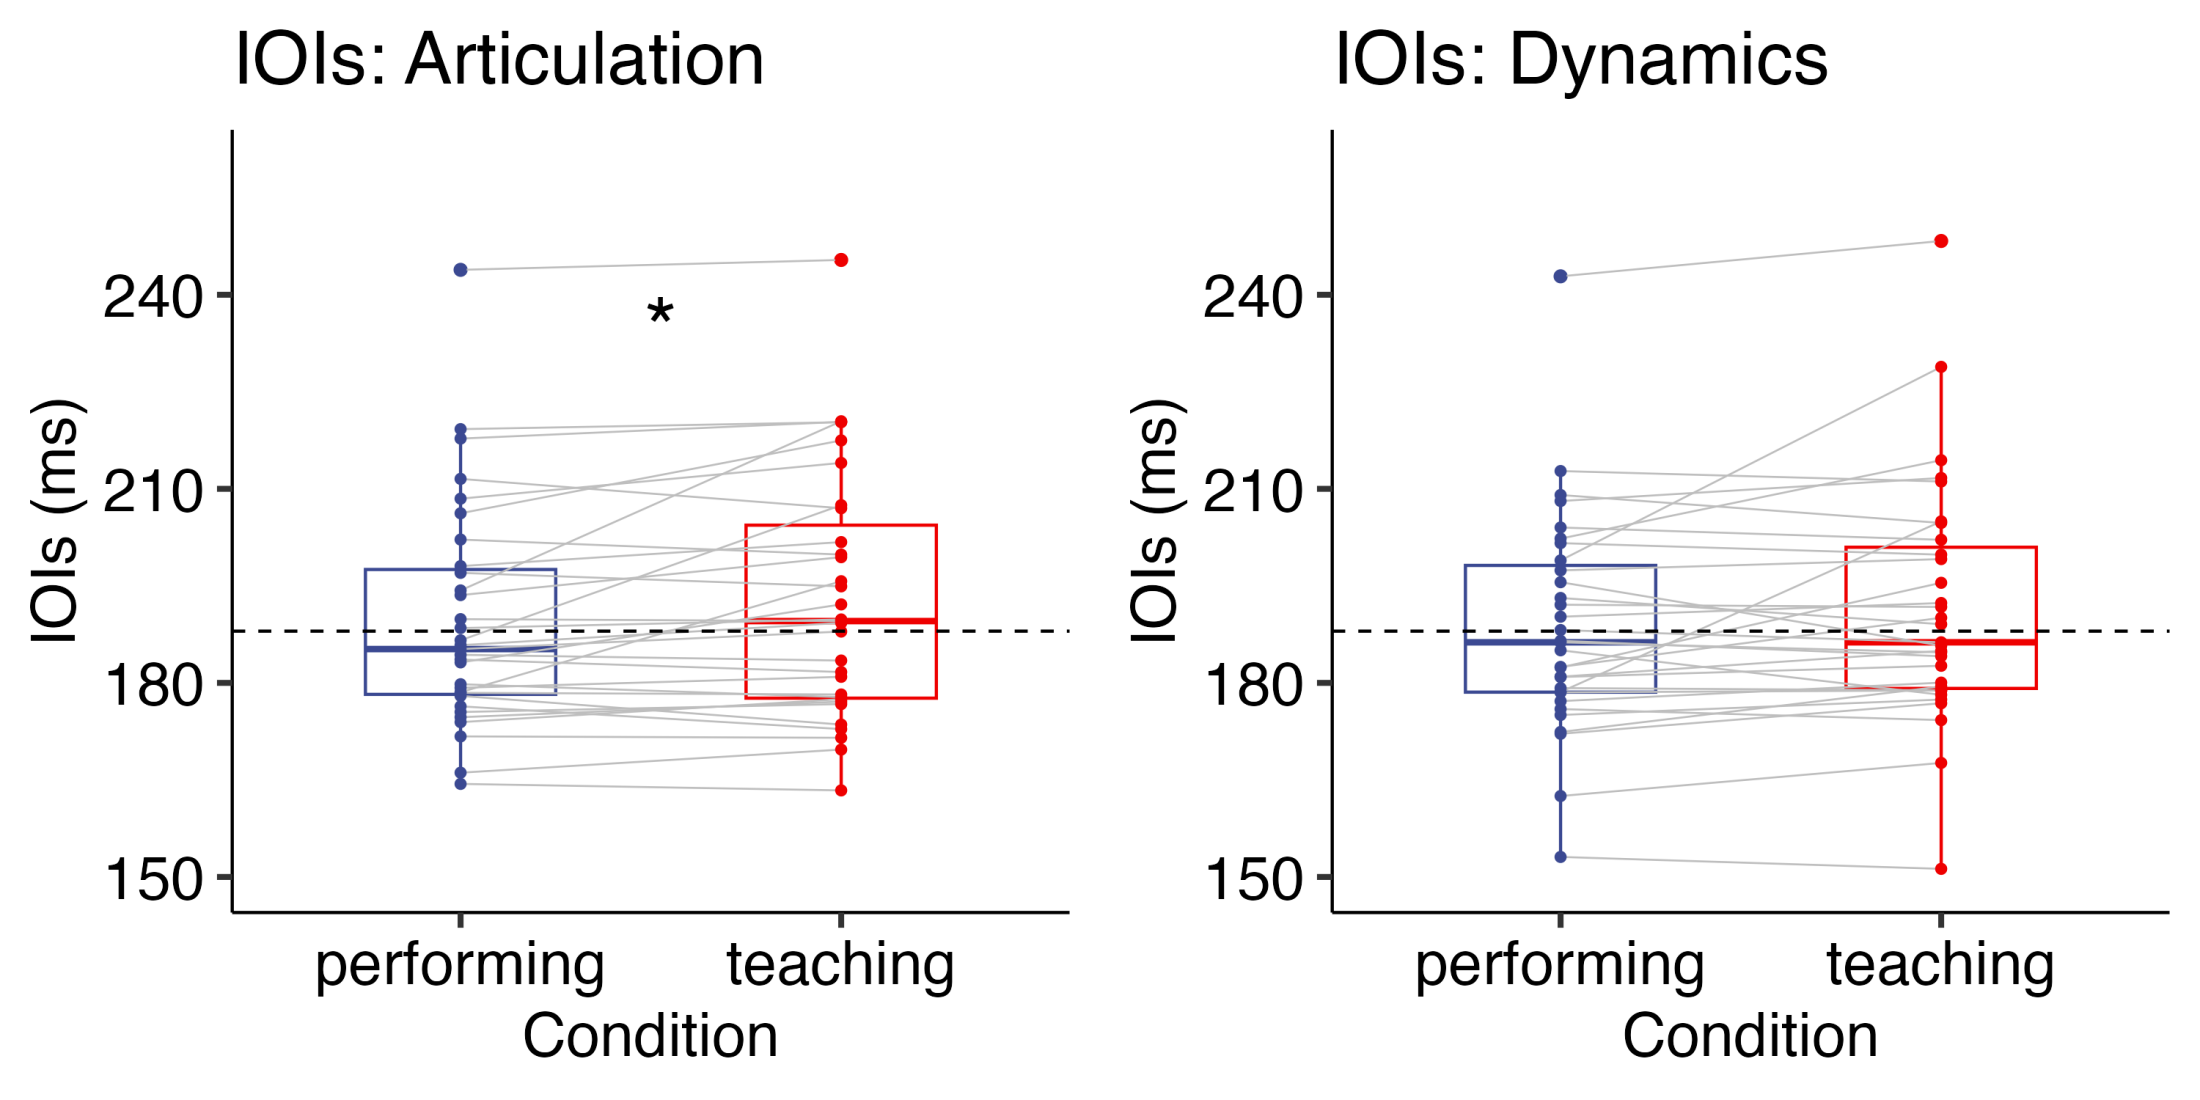
\includegraphics[width=1\linewidth]{manuscript_files/figure-latex/plot-ioi-1-1} \caption{\label{fig:ioi-1}Experiment 1: IOIs (ms) when playing the piece with either articulation (left) or dynamics (right). Each box indicates the IQR with the median, and whiskers extend to a maximum of 1.5 × IQR beyond the box. Significance levels: * \textit{p} < .05, ** \textit{p} < .01, *** \textit{p} < .001}\label{fig:plot-ioi-1}
\end{figure}

\begin{figure}
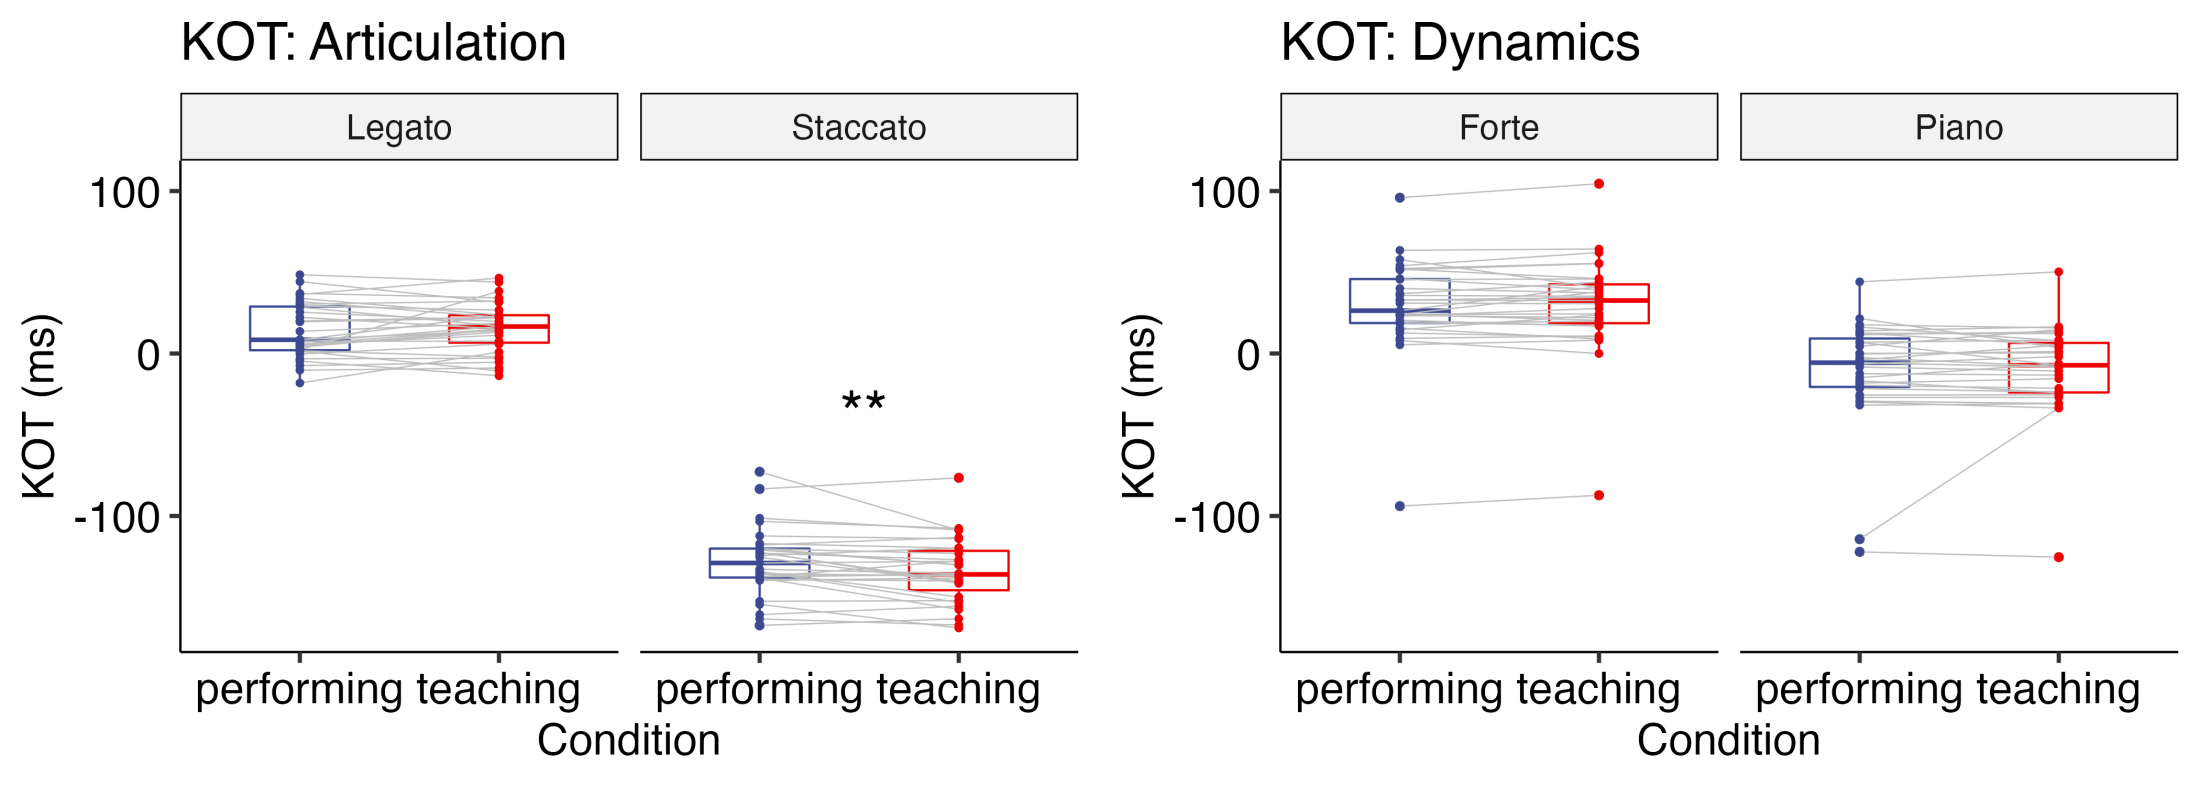
\includegraphics[width=1\linewidth]{manuscript_files/figure-latex/plot-kot-1-1} \caption{\label{fig:kot-1}Experiment 1: KOT (ms) when playing the piece with either articulation (left) or dynamics (right). Each box indicates the IQR with the median, and whiskers extend to a maximum of 1.5 × IQR beyond the box. Significance levels: * \textit{p} < .05, ** \textit{p} < .01, *** \textit{p} < .001}\label{fig:plot-kot-1}
\end{figure}

\hypertarget{discussion}{%
\subsection{2.4. Discussion}\label{discussion}}

\newpage

\hypertarget{experiment-2}{%
\section{3. Experiment 2}\label{experiment-2}}

\hypertarget{method-1}{%
\subsection{3.1. Method}\label{method-1}}

\hypertarget{participants-1}{%
\subsubsection{3.1.1. Participants}\label{participants-1}}

We recruited 21 piano experts who already had a degree in (above bachelor or equivalent) in piano performance/teaching or were studying piano performance at a music school at the time of recruitment. For data analysis, we excluded 1 participants due to insufficient motor skills (1) and an overall deviated tempo (1). Nineteen participants (9 female) were included in data analysis. Most participants were right-handed (left; 2). They had 15.65 years of practice on average (\emph{SD} = 5.67).

\hypertarget{apparatus-and-stimuli-1}{%
\subsubsection{3.1.2. Apparatus and stimuli}\label{apparatus-and-stimuli-1}}

The same apparatus as Experiment 1 was used. We selected Clementi's Sonatina Op.36 (No.3) in C major as a stimulus because it contained our targeted expressions (i.e., articulation, dynamics) and was relatively simple in terms of motor skills. The first 12 measures of the original piece was used and modified so that it had the almost equal number of data points for each dependent variable. The stimulus consisted of a 12-measure isochronous melody notated in 4/4 meter. Non-expressive sheet was used for the purpose of practice (\emph{Figure \ref{fig:stimuli-2}, A}). Expressive notations were added to the non-expressive sheet music for the experiment (\emph{Figure \ref{fig:stimuli-2}, B-C}). These excerpts were confirmed to be musically natural by a doctoral student in piano performance at Liszt Ferenc Academy of Music in Hungary. The fingering was also assigned and confirmed by the same doctoral student.

\hypertarget{procedure-2}{%
\subsubsection{3.1.3. Procedure}\label{procedure-2}}

We employed the same procedure as Experiment 1 with several modifications. First, all participants were required to memorise the piece without expressive notations (i.e., \emph{Figure \ref{fig:stimuli-2}, A}) prior to the experiment. Second, we modified the wording of instructions for the performing condition so that both instructions had the same focus on expressive notations (see details in \emph{\protect\hyperlink{supplemental}{Supplemental Materials}}). Third, participants could choose their preferred tempo from one of the 3 options (100, 110 and 120 beats per minute) as a leading metronome. In order to make sure that participants memorised the piece and had sufficient motor skills, we asked participants to perform the piece without looking at the non-expressive sheet music. As Experiment 1, those who could not perform the piece twice consecutively within 5 attempts were excluded from data analysis. The rest of the procedure was identical to Experiment 1.

\hypertarget{design-and-data-analysis-1}{%
\subsubsection{3.1.4. Design and data analysis}\label{design-and-data-analysis-1}}

Data cleaning, preprocessing and statistical analysis were identical as Experiment 1. For statistical analysis, only 8th notes with expressive notations were included. As a result, only one 8th note in the 4th measure without any expression was not included to calculate dependent variables. Also, IOIs were normalised by their preferred tempo because each participant chose different tempi from the 3 options. Three trials were entirely excluded from data analysis because participants did not follow sheet music. With the same method as Experiment 1, pitch errors were removed manually. For onsets, 3.32\% of the trials contained at least one pitch error (extra notes; 1.66\%, missing notes; 1.57\%, substituted notes; 0.09\%). For offsets, 5.11\% of the trials contained at least one pitch error (extra notes; 1.66\%, missing notes; 1.57\%, substituted notes; 1.88\%). Removed outliers (i.e., responses outside 3 standard deviations from the mean) were less than 5\% of overall responses for each dependent variable.

\begin{figure}
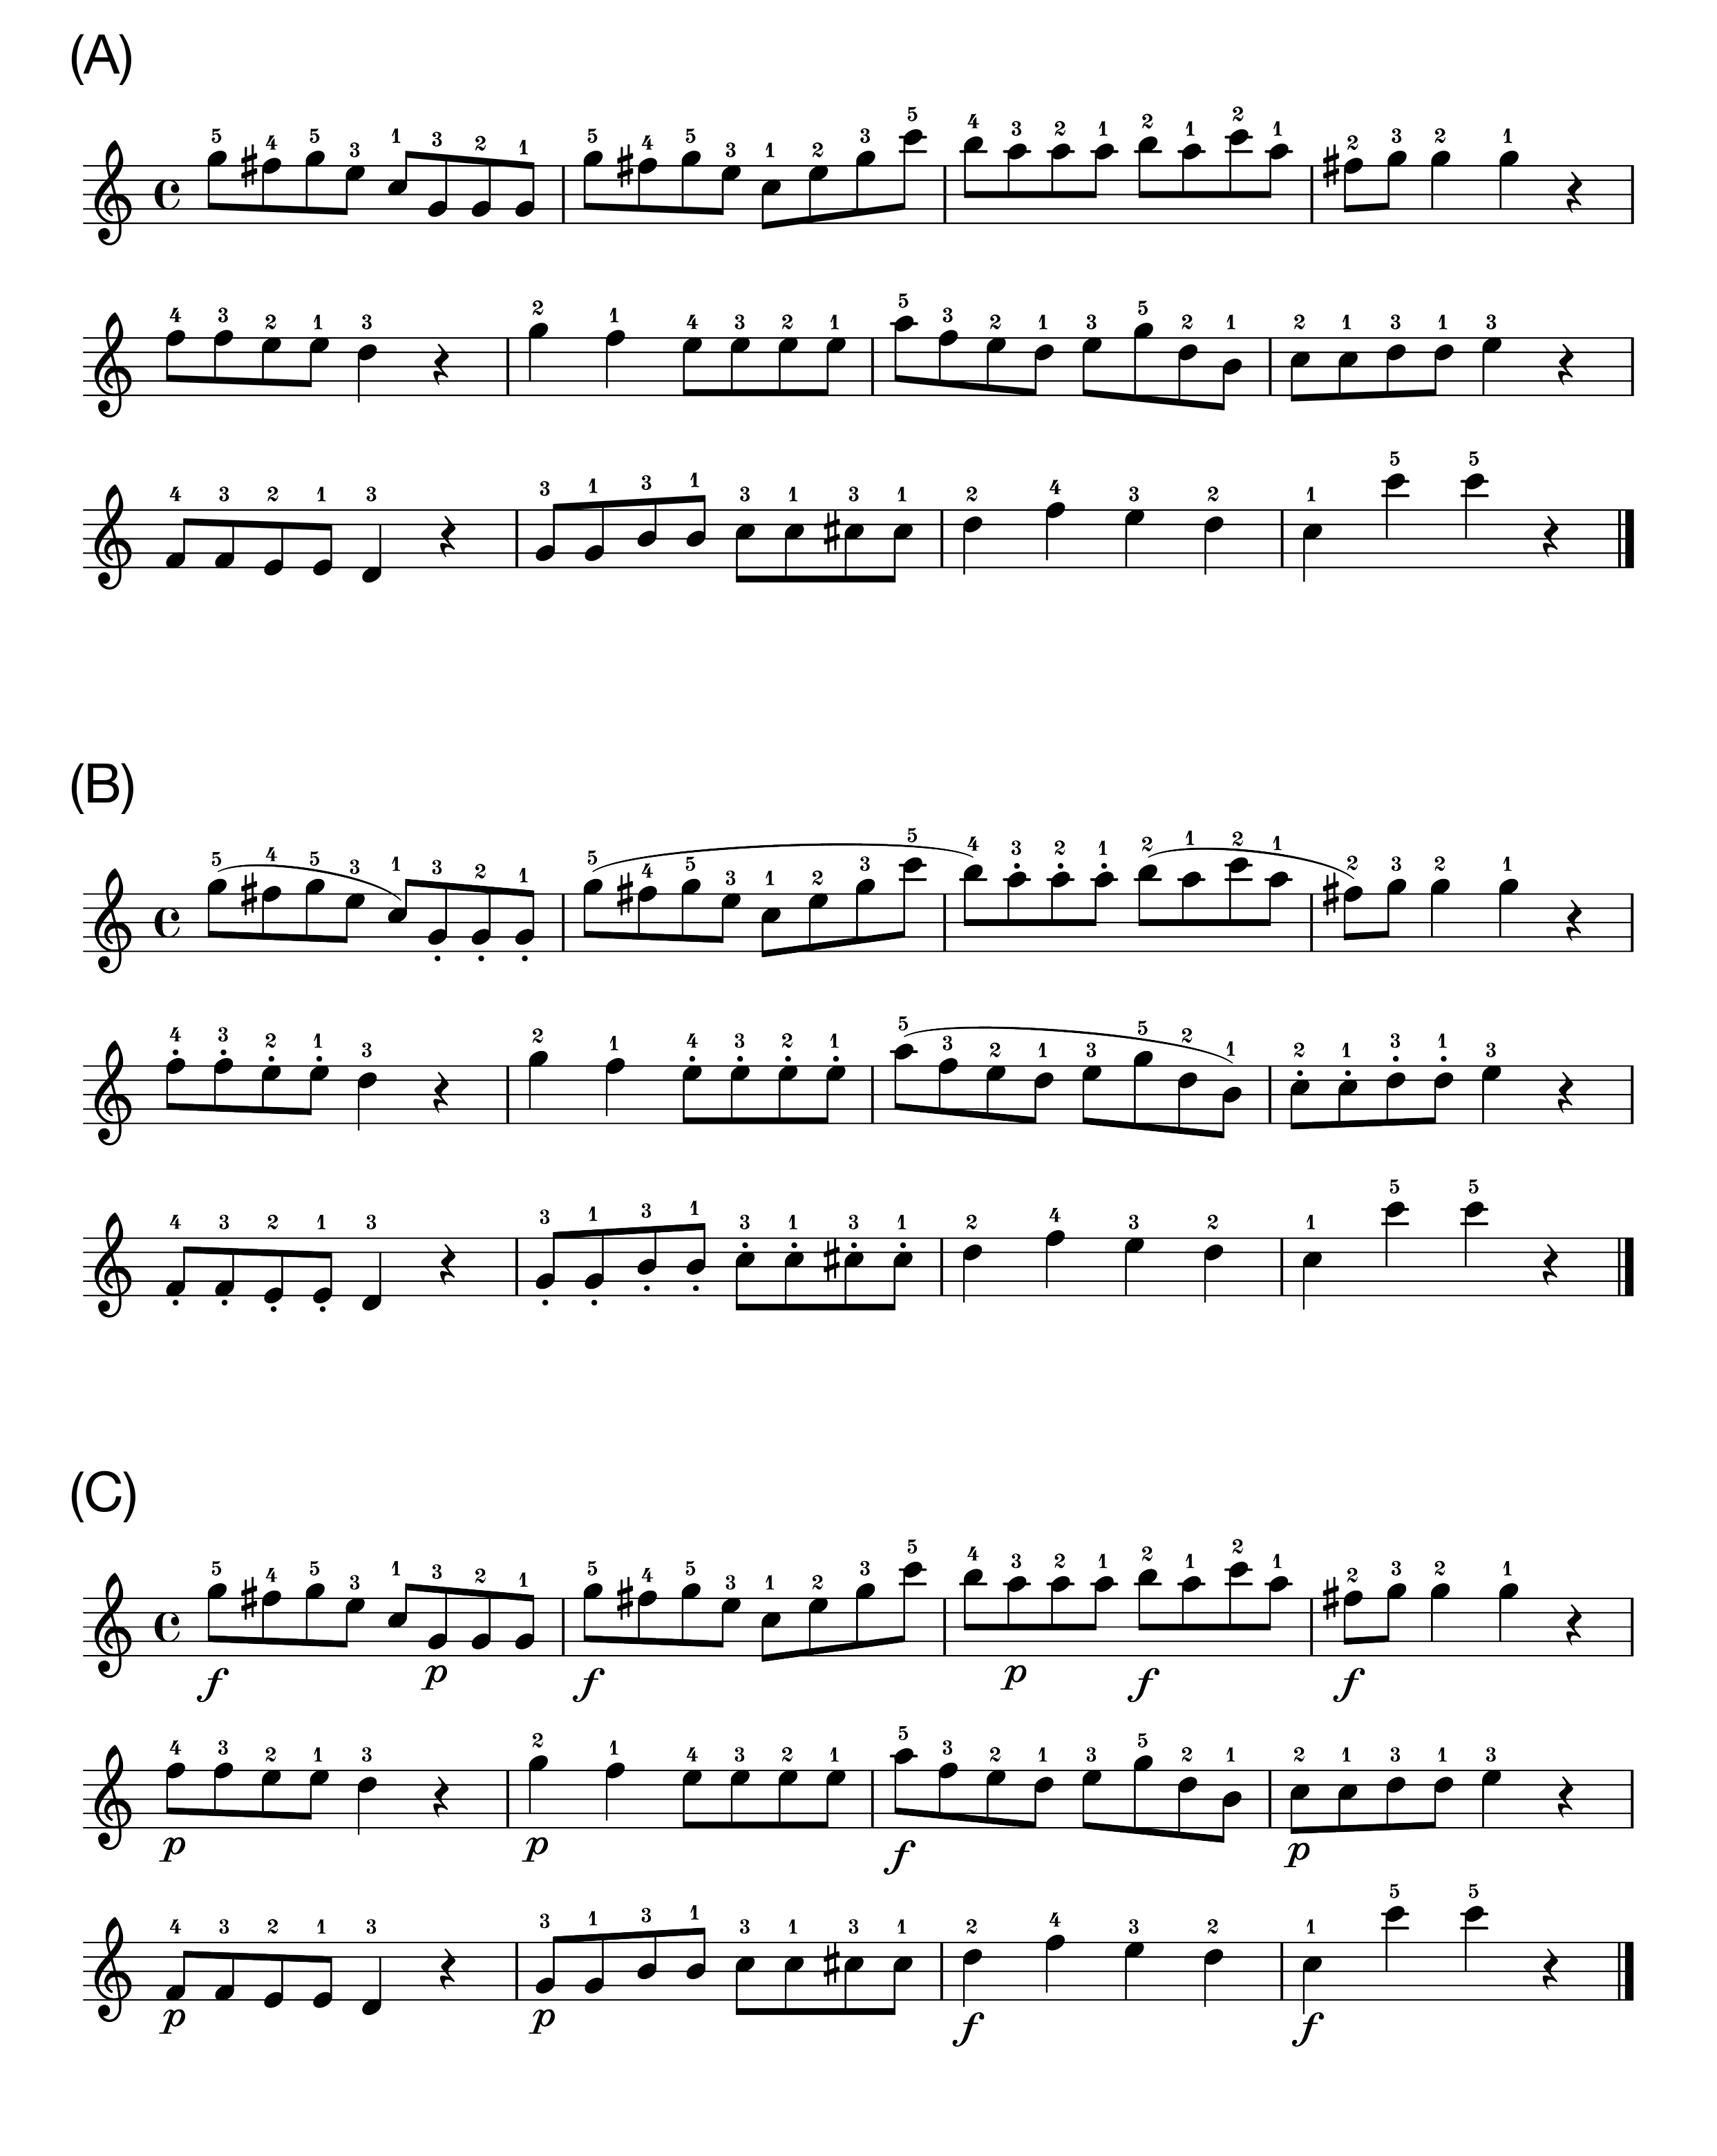
\includegraphics[width=1\linewidth]{manuscript_files/figure-latex/stim-2-1} \caption{\label{fig:stimuli-2}(A)Non-expressive sheet music. (B)Articulation. The curved line (slur) indicates legato and the dots indicate staccato. (C)Dynamics. The symbol `f' denotes forte and the symbol `p' denotes piano. For data analysis, only the 8th notes were included.}\label{fig:stim-2}
\end{figure}

\hypertarget{results-articulation-1}{%
\subsection{3.2. Results (Articulation)}\label{results-articulation-1}}

As Experiment 1, we first report results for performance the piece with the notated expression of articulation (\emph{Figure \ref{fig:stimuli-2}, B}). followed by performance of the piece with the notated expression of dynamics (\emph{Figure \ref{fig:stimuli-2}, C}).

\hypertarget{interonset-intervals-iois-2}{%
\subsubsection{3.2.1. Interonset Intervals (IOIs)}\label{interonset-intervals-iois-2}}

A paired-sample \emph{t}-test showed that participants played more slowly in the teaching condition {[}\emph{M} = 0.972, \emph{SD} = 0.042{]} than in the performing condition {[}\emph{M} = 0.958, \emph{SD} = 0.034{]} while playing the piece with notated articulation (\emph{t}(18) = 2.64
, \emph{p} = 0.017; \emph{Figure \ref{fig:ioi-2}}). A Wiscoxon Signed-rank test also confirmed that there was a significant difference between the two condition (\emph{p} = 0.026).

\hypertarget{key-overlap-ratio-kor}{%
\subsubsection{3.2.2. Key-Overlap Ratio (KOR)}\label{key-overlap-ratio-kor}}

Blah

\hypertarget{key-velocity-kv-2}{%
\subsubsection{3.2.3. Key Velocity (KV)}\label{key-velocity-kv-2}}

Blah

\hypertarget{kv-transition-points-2}{%
\subsubsection{3.2.4. KV Transition Points}\label{kv-transition-points-2}}

Blah

\hypertarget{results-dynamics-1}{%
\subsection{3.3. Results (Dynamics)}\label{results-dynamics-1}}

\hypertarget{interonset-intervals-iois-3}{%
\subsubsection{3.3.1. Interonset Intervals (IOIs)}\label{interonset-intervals-iois-3}}

A paired-sample \emph{t}-test showed no significant difference between the teaching condition {[}\emph{M} = 0.962, \emph{SD} = 0.041{]} and the performing condition {[}\emph{M} = 0.961, \emph{SD} = 0.037{]} while playing the piece with notated articulation (\emph{t}(18) = 0.37, \emph{p} = 0.719; \emph{Figure \ref{fig:ioi-2}}). A Wiscoxon Signed-rank test also confirmed that there was no significant difference between the two condition (\emph{p} = 0.922).

\hypertarget{key-velocity-kv-3}{%
\subsubsection{3.3.2. Key Velocity (KV)}\label{key-velocity-kv-3}}

Blah

\hypertarget{kv-transition-points-3}{%
\subsubsection{3.3.3. KV Transition Points}\label{kv-transition-points-3}}

Blah

\hypertarget{key-overlap-ratio-kor-1}{%
\subsubsection{3.3.4. Key-Overlap Ratio (KOR)}\label{key-overlap-ratio-kor-1}}

Blah

\begin{figure}
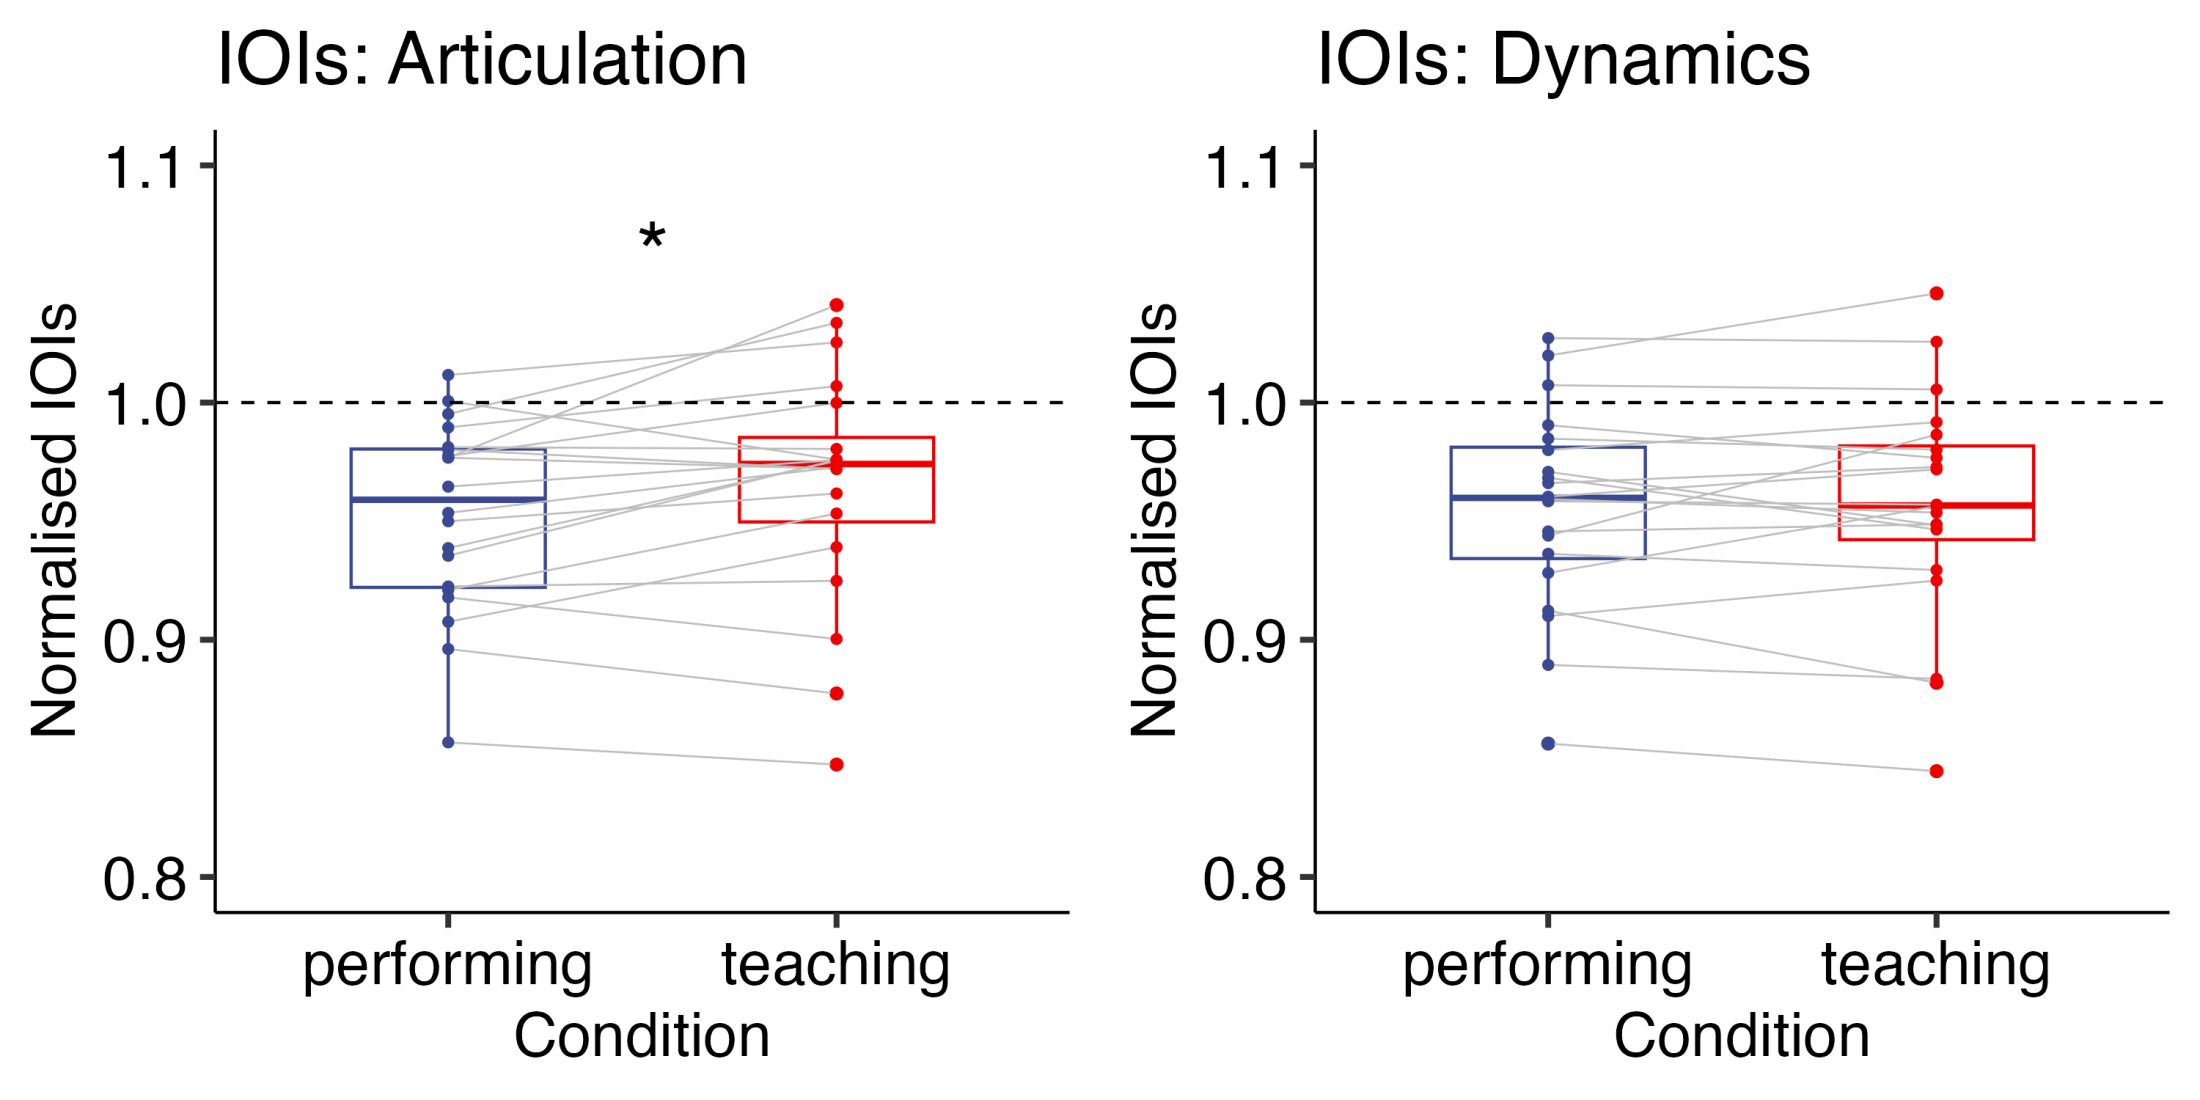
\includegraphics[width=1\linewidth]{manuscript_files/figure-latex/plot-ioi-2-1} \caption{\label{fig:ioi-2}Experiment 2: Normalised IOIs when playing the piece with either articulation (left) or dynamics (right). Each box indicates the IQR with the median, and whiskers extend to a maximum of 1.5 × IQR beyond the box. Significance levels: * \textit{p} < .05, ** \textit{p} < .01, *** \textit{p} < .001}\label{fig:plot-ioi-2}
\end{figure}

\begin{figure}
\includegraphics[width=1\linewidth]{manuscript_files/figure-latex/plot-kot-2-1} \caption{\label{fig:kot-1}Experiment 2: KOR when playing the piece with either articulation (left) or dynamics (right). Each box indicates the IQR with the median, and whiskers extend to a maximum of 1.5 × IQR beyond the box. Significance levels: * \textit{p} < .05, ** \textit{p} < .01, *** \textit{p} < .001}\label{fig:plot-kot-2}
\end{figure}

\hypertarget{discussion-1}{%
\subsection{3.4. Discussion}\label{discussion-1}}

\newpage

\hypertarget{general-discussion}{%
\section{4. General Discussion}\label{general-discussion}}

\hypertarget{acknowledgements}{%
\section{Acknowledgements}\label{acknowledgements}}

We thank Dávid Csűrös for his help with data collection. This research was supported by the European Research Council under the European Union's Seventh Framework Program (FP7/2007-2013)/ERC (European Research Council) grant agreement no. 609819, SOMICS, and by ERC grant agreement no. 616072, JAXPERTISE.

\hypertarget{declarations-of-interest}{%
\section{Declarations of interest}\label{declarations-of-interest}}

All authors have no conflict of interest.

\newpage

\hypertarget{references}{%
\section{References}\label{references}}

\begingroup
\setlength{\parindent}{-0in}
\setlength{\leftskip}{0in}

\hypertarget{refs}{}
\begin{cslreferences}
\leavevmode\hypertarget{ref-brand_2002}{}%
Brand, R. J., Baldwin, D. A., \& Ashburn, L. A. (2002). Evidence for ``motionese'': Modifications in mothers' infant-directed action. \emph{Developmental Science}, \emph{5}(1), 72--83. \url{https://doi.org/10.1111/1467-7687.00211}

\leavevmode\hypertarget{ref-bresin_2000}{}%
Bresin, R., \& Battel, G. U. (2000). Articulation Strategies in Expressive Piano Performance Analysis of Legato, Staccato, and Repeated Notes in Performances of the Andante Movement of Mozart's Sonata in G Major (K 545). \emph{Journal of New Music Research}, \emph{29}(3), 211--224. \url{https://doi.org/10.1076/jnmr.29.3.211.3092}

\leavevmode\hypertarget{ref-campisi_2013}{}%
Campisi, E., \& Özyürek, A. (2013). Iconicity as a communicative strategy: Recipient design in multimodal demonstrations for adults and children. \emph{Journal of Pragmatics}, \emph{47}(1), 14--27. \url{https://doi.org/10.1016/j.pragma.2012.12.007}

\leavevmode\hypertarget{ref-csibra_2009}{}%
Csibra, G., \& Gergely, G. (2009). Natural pedagogy. \emph{Trends in Cognitive Sciences}, \emph{13}(4), 148--153. \url{https://doi.org/10.1016/j.tics.2009.01.005}

\leavevmode\hypertarget{ref-fernald_1985}{}%
Fernald, A. (1985). Four-month-old infants prefer to listen to motherese. \emph{Infant Behavior and Development}, \emph{8}(2), 181--195. \url{https://doi.org/10.1016/S0163-6383(85)80005-9}

\leavevmode\hypertarget{ref-fukuyama_2015}{}%
Fukuyama, H., Qin, S., Kanakogi, Y., Nagai, Y., Asada, M., \& Myowa-Yamakoshi, M. (2015). Infant's action skill dynamically modulates parental action demonstration in the dyadic interaction. \emph{Developmental Science}, \emph{18}(6), 1006--1013. \url{https://doi.org/10.1111/desc.12270}

\leavevmode\hypertarget{ref-NIPS2016_6413}{}%
Ho, M. K., Littman, M., MacGlashan, J., Cushman, F., \& Austerweil, J. L. (2016). Showing versus doing: Teaching by demonstration. In D. D. Lee, M. Sugiyama, U. V. Luxburg, I. Guyon, \& R. Garnett (Eds.), \emph{Advances in neural information processing systems 29} (pp. 3027--3035). Curran Associates, Inc.

\leavevmode\hypertarget{ref-juslin_2003}{}%
Juslin, P. N. (2003). Five Facets of Musical Expression: A Psychologist's Perspective on Music Performance. \emph{Psychology of Music}, \emph{31}(3), 273--302. \url{https://doi.org/10.1177/03057356030313003}

\leavevmode\hypertarget{ref-mcellin_2017}{}%
McEllin, L., Knoblich, G., \& Sebanz, N. (2017). Distinct kinematic markers of demonstration and joint action coordination? Evidence from virtual xylophone playing. \emph{Journal of Experimental Psychology: Human Perception and Performance}, \emph{44}(6), 885. \url{https://doi.org/10.1037/xhp0000505}

\leavevmode\hypertarget{ref-schaik_2019}{}%
Schaik, J. E. van, Meyer, M., Ham, C. R. van, \& Hunnius, S. (2019). Motion tracking of parents' infant- versus adult-directed actions reveals general and action-specific modulations. \emph{Developmental Science}, \emph{0}(0), e12869. \url{https://doi.org/10.1111/desc.12869}

\leavevmode\hypertarget{ref-sloboda_2000}{}%
Sloboda, J. A. (2000). Individual differences in music performance. \emph{Trends in Cognitive Sciences}, \emph{4}(10), 397--403. \url{https://doi.org/10.1016/S1364-6613(00)01531-X}

\leavevmode\hypertarget{ref-tomasello_2016}{}%
Tomasello, M. (2016). The ontogeny of cultural learning. \emph{Current Opinion in Psychology}, \emph{8}, 1--4. \url{https://doi.org/10.1016/j.copsyc.2015.09.008}

\leavevmode\hypertarget{ref-uther_2007}{}%
Uther, M., Knoll, M. A., \& Burnham, D. (2007). Do you speak E-NG-L-I-SH? A comparison of foreigner- and infant-directed speech. \emph{Speech Communication}, \emph{49}(1), 2--7. \url{https://doi.org/10.1016/j.specom.2006.10.003}

\leavevmode\hypertarget{ref-whiten_2017}{}%
Whiten, A. (2017). Social Learning and Culture in Child and Chimpanzee. \emph{Annual Review of Psychology}, \emph{68}(1), 129--154. \url{https://doi.org/10.1146/annurev-psych-010416-044108}
\end{cslreferences}

\endgroup
\raggedbottom

\end{document}
